\documentclass{beamer}
\usepackage[polish]{babel}                      % Język polski
\usepackage[utf8]{inputenc}                     % Kodowanie dokumentu
\usepackage[T1]{fontenc}                        % Kodowanie fontów
\usepackage{times}
%\usepackage{graphicx}

\title{ConvML}
\author{Marcin Kacprzak\\
marcin.kacprzak@entertech.com.pl}
\institute{EnterTECH}
\date{4 listopad 2011}
\usetheme{Warsaw}
%\usecolortheme{beaver}

\begin{document}

\begin{frame}
\titlepage
\end{frame}

\section*{Plan prezentacji}
\begin{frame}
\tableofcontents
\end{frame}

\section{Składnia}

\subsection{Struktura przenośnika}
\begin{frame}
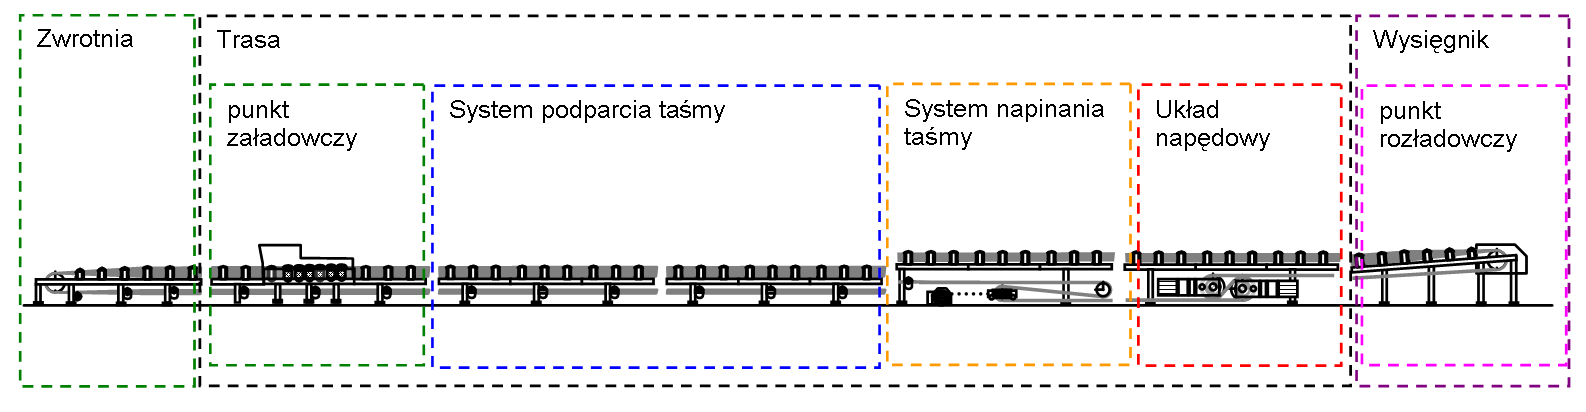
\includegraphics[width=\textwidth]{beamer/struktura}

\pause

\begin{center}
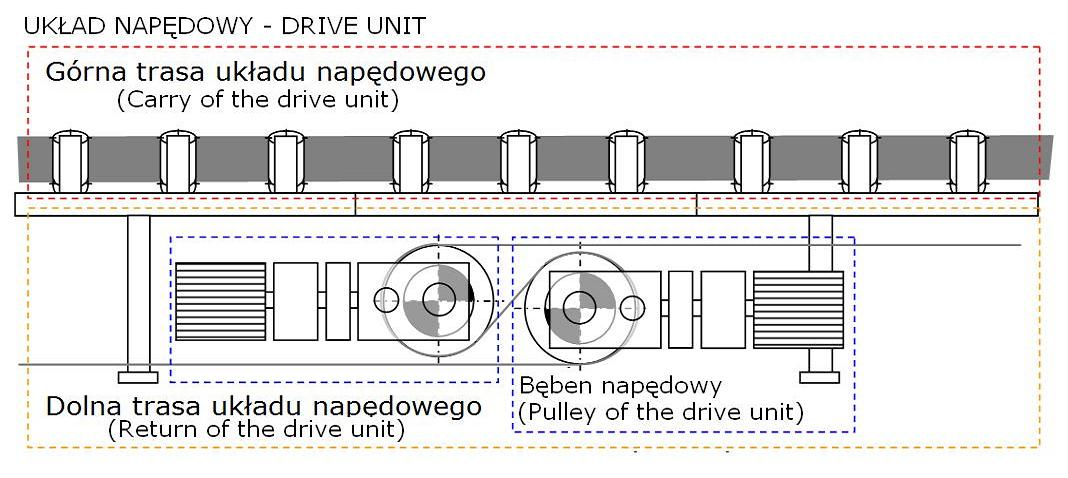
\includegraphics[width=0.7\textwidth]{beamer/drive_unit}
\end{center}
\end{frame}

\subsection{Dekompozycja przenosnika}
\begin{frame}
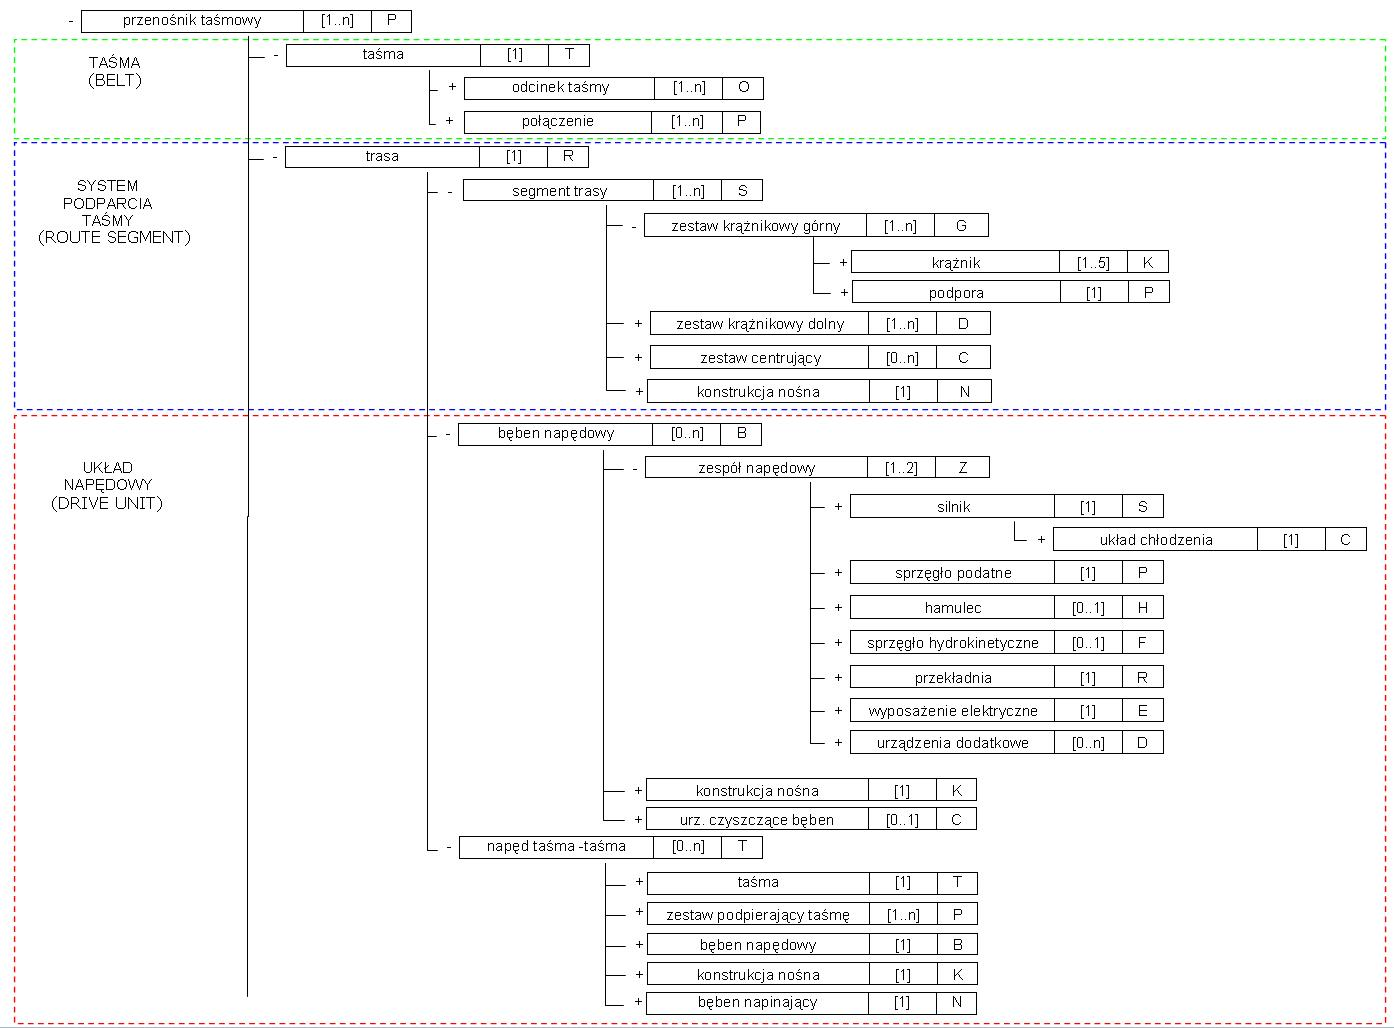
\includegraphics[width=\textwidth]{beamer/struktura_word}
\end{frame}

\subsection{Narzędzia informatyczne}
\begin{frame}
\begin{itemize}
\item Przenośnik taśmowy można w naturalny sposób opisać modelem
  hierarchicznym.
\item Jako format zapisu danych wybrano język XML ze względu na:
\begin{itemize}
  \item tekstowy, czytelny dla człoweka zapis danych w pliku,
  \pause\item dopracowane narzędzia walidacji dokumentów (XML Schema),
  \pause\item dostępność dobrej jakości bibliotek na różne platformy
    informatyczne,
  \pause\item możliwość rozbudowy języka bez utraty wstecznej
    kompatybilności,
  \pause\item zaawansowane przesukiwanie danych za pomocą XPath/XQuery,
%  \item możliwość osadzania dokumentów w innych dokumentach XML,
  \item możliwosć transformacji do innych formatów za pomocą XSLT.
\end{itemize}
\end{itemize}
\end{frame}

\begin{frame}
\frametitle{Konwencje}
\begin{itemize}
\item Elementy XML odpowiadają obiektom modelu,
\item atrybuty XML odpowiadają właściwościom obiektów,
\item brak wykorzystania węzłów tekstowych.
\end{itemize}
\end{frame}

\begin{frame}
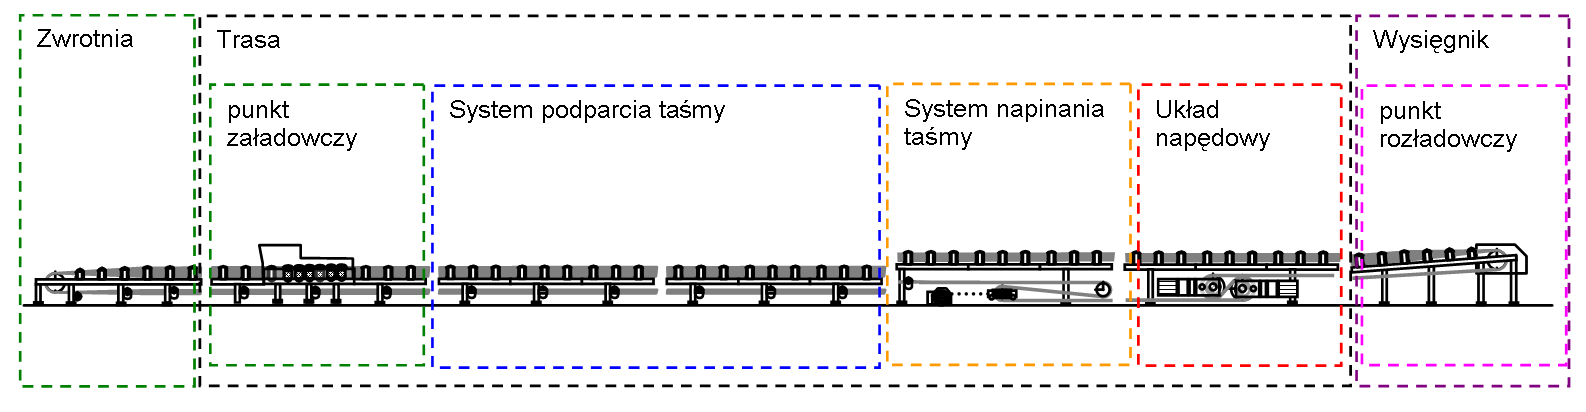
\includegraphics[width=\textwidth]{beamer/struktura}

\pause

\begin{center}
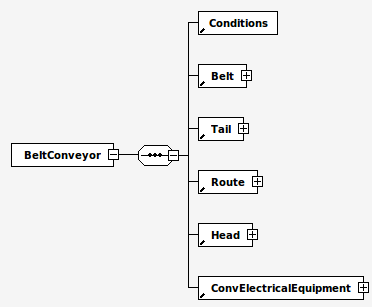
\includegraphics[width=0.5\textwidth]{png/przenosnik_xsd}
\end{center}
\end{frame}

\section{Przykłady}
\subsection{Root}
\begin{frame}[fragile]
%\begin{example}
\begin{verbatim}
<?xml version="1.0" encoding="UTF-8"?>
<ConvML version="1.2"
        xmlns="http://www.entertech.com.pl/convml">
  <Meta/>
  <Types/>
  <BeltConveyor>
    <Conditions/>
    <Belt/>
    <Tail/>
    <Route/>
    <Head/>
    <ConvElectricalEquipment/>
  </BeltConveyor>
</ConvML>
\end{verbatim}
%\end{example}
\end{frame}

\subsection{Taśma}
\begin{frame}
\frametitle{Taśma}
\begin{center}
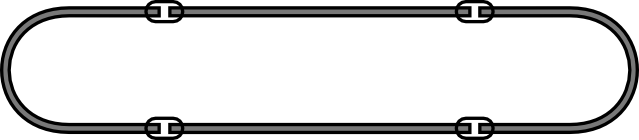
\includegraphics[width=0.5\textwidth]{png/tasma}

\pause

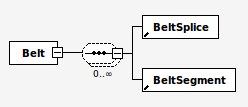
\includegraphics[width=0.5\textwidth]{png/tasma_xsd}
\end{center}
\end{frame}

\begin{frame}[fragile]
%\begin{example}
\begin{verbatim}
<Belt>
  <BeltSplice id="1" />
  <BeltSegment id="2" />
  <BeltSplice id="3" />
  <BeltSegment id="4" />
  <BeltSplice id="5" />
  <BeltSegment id="6" />
</Belt>
\end{verbatim}
%\end{example}
\end{frame}

\begin{frame}[fragile]
%\begin{example}
\begin{verbatim}
<Belt>
  <BeltSplice spliceStrength="1000" />
  <BeltSegment type="GTP-1200/t"
               length="100"
               productionDate="2005-04-11"
               certificate="1257"/>
  <BeltSplice spliceStrength="1000" />
  <BeltSegment type="GTP-1200/t"
               length="100"
               productionDate="2005-07-15"
               certificate="1258"/>
</Belt>
\end{verbatim}
%\end{example}
\end{frame}

\subsection{Trasa}
\begin{frame}
\begin{center}
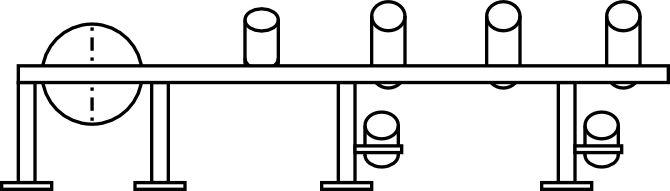
\includegraphics[width=0.5\textwidth]{png/zwrotnia}~~~~
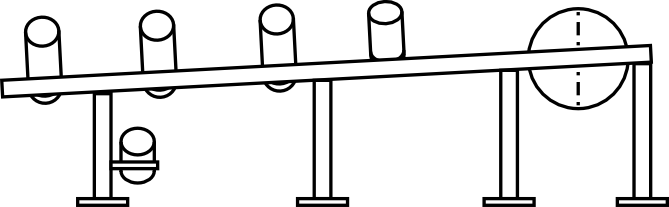
\includegraphics[width=0.5\textwidth]{png/wysiegnik}

\pause

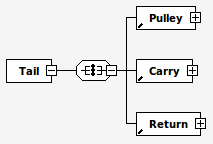
\includegraphics[width=0.3\textwidth]{png/zwrotnia_xsd}~~~~
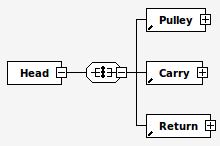
\includegraphics[width=0.3\textwidth]{png/wysiegnik_xsd}

\end{center}
\end{frame}

\begin{frame}
\begin{center}
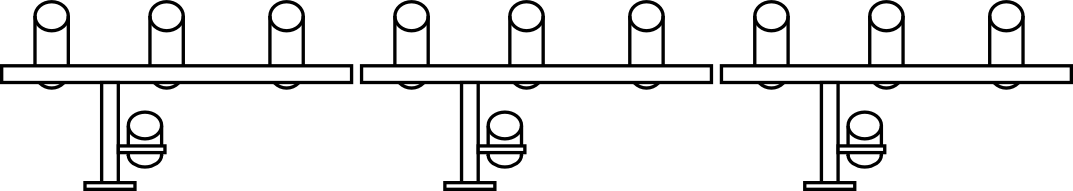
\includegraphics[width=0.7\textwidth]{png/odcinek_trasy}

\pause

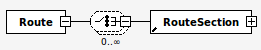
\includegraphics[width=0.4\textwidth]{png/trasa_xsd}

\pause

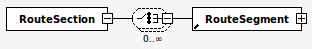
\includegraphics[width=0.4\textwidth]{png/odcinek_trasy_xsd}

\pause

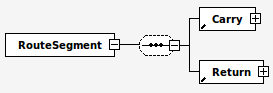
\includegraphics[width=0.4\textwidth]{png/segment_trasy_xsd}
\end{center}
\end{frame}

\begin{frame}[fragile]
\begin{verbatim}
<Tail>
    <Pulley/>
    <Carry/>
    <Return/>
</Tail>
<Route>
    <RouteSection length="50">
        <RouteSegment>
            <Carry/>
            <Return/>
        </RouteSegment>
    </RouteSection>
    <RouteSection angle="5" length="100"/>
    <RouteSection length="50"/>
</Route>
\end{verbatim}
\end{frame}

\begin{frame}[fragile]
\begin{verbatim}
<Head>
    <Pulley>
        <DriveUnit>
            <Motor/>
            <Coupling/>
            <Gearbox/>
            <ElectricalEquipment/>
        <DriveUnit/>
    </Pulley>
    <Carry/>
    <Return/>
</Head>
\end{verbatim}
\end{frame}

\subsection{Typy}
\begin{frame}
\frametitle{Typy}
Część właściwości obiektów takich jak:
\begin{itemize}
\item odcinek taśmy
\item silnik,
\item przekładnia,
\item bęben,
\end{itemize}
można zdefinować w typie zamiast instancjach.
\end{frame}

\begin{frame}[fragile]
\begin{verbatim}
<Types>
  <BeltSegmentType typeId="GTP-1200/t"
                   bottomCoverThickness="2"
                   carcassType="tekstylny"
                   coverDescription="trudnopalna"
                   elasticityModulus="2000"
                   manufacturer="Wolbrom"
                   pliesNumber="3"
                   topCoverThickness="4"
                   width="1200"/>
</Types>
\end{verbatim}
\end{frame}

\begin{frame}[fragile]
\begin{verbatim}
<Belt>
  <BeltSplice/>
  <BeltSegment type="GTP-1200/t"
               length="100"
               productionDate="2005-04-11"
               certificate="1257"/>
  <BeltSplice/>
  <BeltSegment type="GTP-1200/t"
               length="100"
               productionDate="2005-07-15"
               certificate="1258"/>
</Belt>
\end{verbatim}
\end{frame}


\section{Podsumowanie}
\begin{frame}
Dzięki strukturze języka ConvML nastawionej na czytelność możliwe było
bezpośrednie odzwierciedlenie hierarchi obiektów na interfejs
użytkownika.
\end{frame}

\begin{frame}
\begin{center}
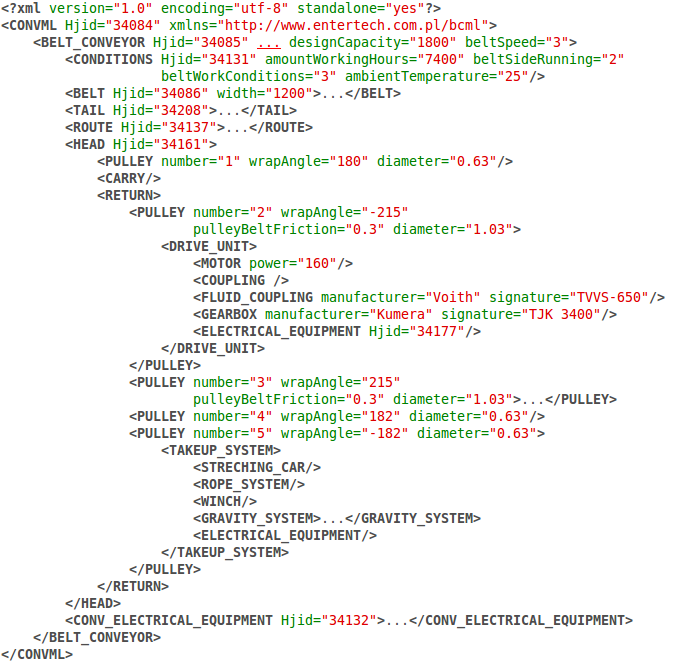
\includegraphics[width=0.5\textwidth]{beamer/Zaznaczenie_026}
\pause
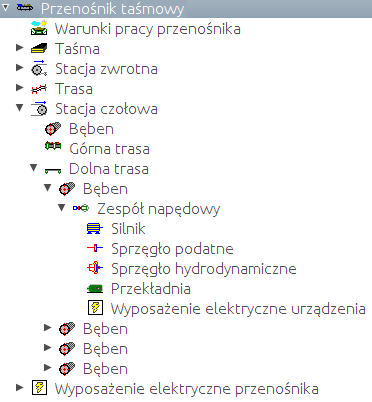
\includegraphics[width=0.5\textwidth]{beamer/Zaznaczenie_024}
\end{center}
\end{frame}

\begin{frame}
\begin{itemize}
\item Język ConvML został wykorzystany w aplikacji BCE$^{KGHM}$,
  gdzie jest podstawowym formatem zapisu projektów.

\item Obiektowa (DOM) postać języka ConvML jest wykorzystywana przez
  aplikację BCE podczas tworzenia i modyfikowania projektów
  przenośników.

\item Współpracująca z programem BCE$^{KGHM}$ baza danych pracuje
  na relacyjnym odwzorowaniu struktury języka ConvML.
\end{itemize}
\end{frame}

\begin{frame}
\begin{center}
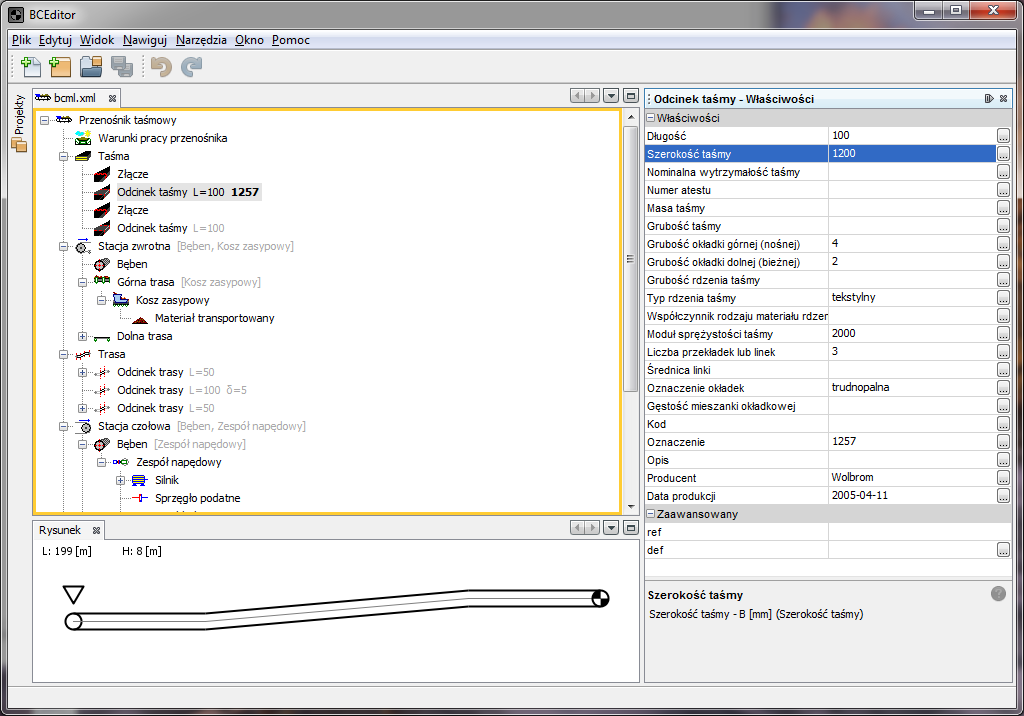
\includegraphics[width=\textwidth]{beamer/mainWin}
\end{center}
\end{frame}

\begin{frame}
W wersja 1.2 języka ConvML najważniejsze zmiany to:
\item typy,
\item dokładne współrzędne geometryczne bębnów,
\item powiązanie punktów rozładowczych i koszy zasypowych pomiędzy
  przenosnikami.
\end{frame}

\end{document}

